\chapter{证明器的总体设计}
\label{chap:struct}
本章给出证明器的总体设计,并说明证明器的各个部分之间如何协作证明一个命题。

\section{输入语言}
本文设计的证明器需要证明的命题可以分成两部分:一部分是纯的一阶逻辑及其理论,另一部分是分离逻辑。前者主要表达程序中变量、函数之间的相等和不等关系,后者主要表示程序中数据结构的变化。

两者在各自推理的同时,前者也为后者服务,如向后者提供指针运算、指针相等关系等内容。这决定了证明器要支持一阶逻辑中的算术理论和相等理论。

由上述需求,我们设计的命题语言如图\ref{struct:syntax}所示。

\begin{figure}[!htbp]
  \centering
  \begin{tabular}{rrcl}
    整数常元 & $C$ & \sep & $\left\{ 0, 1, -1, \ldots \right\}$ \\
    整型变元 & $X$ & \sep & $\left\{ x_0, x_1, x_2, \ldots \right\}$ \\
    未解释函数 & $F$ & \sep & $\left\{ f_0, f_1, f_2, \ldots \right\}$ \\
    命题变元 & $A$ & \sep & $\left\{ A_0, A_1, \ldots \right\}$ \\
    公式项  & $T$ & \sep & $C$ \deli{} $X$ \deli{} $A$ \deli{} $F(T,$\ldots$,T)$ \deli{} $+(T, T)$ \deli{} $\cdot(C,T)$ \\
    一阶逻辑原子公式 & $Y$ & \sep{} & $T \le T$ \deli{} $T = T$ \deli{} $A$ \deli{} $\mathrm{true}$ \\
    一阶逻辑公式 & $\Pi$ & \sep{} & $Y$ \deli{}  $\lnot \Pi$ \deli{} $\Pi \impl \Pi$ \deli{} $\Pi \land \Pi$ \deli{} $\Pi \lor \Pi$ \\
    分离逻辑原子公式 & $H$ & \sep{} & $T \mapsto T$ \deli{} $\mathrm{emp}$ \\
    分离逻辑公式 & $\Sigma$ & \sep{} & $H$ \deli{} $\Sigma \ast \Sigma$ \\
    命题 & $P$ & \sep & $ \Pi \land \Sigma \impl \Pi' \land \Sigma' $
  \end{tabular}
  \caption{命题语言的语法}
  \label{struct:syntax}
\end{figure}

证明器接受的命题的整体是一个蕴含式,前件和后件都分别由$\Pi$和$\Sigma$两部分构成,分别代表一阶逻辑部分和分离逻辑部分。

$\Pi$和$\Pi'$是一个无量词的一阶逻辑公式。二元函数$+$和$\cdot$分别解释为整数环上的加法和数乘运算,这意味着只能支持线性的整数算术;除此之外,可出现有限个有限元的函数,它们是未解释的。

$\Sigma$和$\Sigma'$是包含分离逻辑符号的公式。为简化起见,分离逻辑公式只能用$\ast$(分离合取)联结词连接,原子公式只能是$\mathrm{emp}$和$T_1 \mapsto T_2$的形式,分别代表空堆和仅包含一项的堆。

命题语言语义的定义如图\ref{struct:semantic}。
\begin{figure}[!htbp]
  \centering
  \begin{tabular}{rcl}
    $s, h \models P$ & & \\
    $s$是栈 & & $s: T \impl \mathbb{Z}$ \\
    $h$是堆 & & $h: \mathbb{Z} 	\backslash \{0\} \impl \mathbb{Z}$ \\
    $s, h \models t_1 = t_2$ & $\iff$ & $s(t_1) = s(t_2)$ \\
    $s, h \models t_1 \leq t_2$ & $\iff$ & $s(t_1) \leq s(t_2)$ \\
    $s, h \models \mathrm{true}$ & $\iff$ & 真 \\
    $s, h \models \lnot P$ & $\iff$ & $s, h \models P$为假 \\
    $s, h \models P \impl Q$ & $\iff$ & 若$s, h \models P$,则$s, h \models Q$ \\
    $s, h \models P \land Q$ & $\iff$ & $s, h \models P$ 且 $s, h \models Q$ \\
    $s, h \models P \lor Q$ & $\iff$ & $s, h \models P$ 或 $s, h \models Q$ \\
    $s, h \models \mathrm{emp}$ & $\iff$ & $\mathrm{dom}(h)= \emptyset$ \\
    $s, h \models t_1 \mapsto t_2$ & $\iff$ & $s(t_1) \neq 0$ 且 $\mathrm{dom}(h) = \{s(t_1)\}$ \\
    & & 且 $h(s(t_1)) = s(t_2)$ \\
    $s, h \models P \ast Q$ & $\iff$ & 存在$h1, h2$, $h1 \bot h2$ 且 $h = h1 \ast h2$ \\
    & & 且 $s, h1 \models P$ 且 $s, h2 \models Q$ \\
  \end{tabular}
  \caption{命题语言的语义}
  \label{struct:semantic}
\end{figure}

由于分离逻辑隐式包含了堆,这在纯的一阶逻辑中是没有的。因此图中的语义定义主要说明了一阶逻辑符号拓展到有堆出现时的意义。

\section{结构及流程}

\begin{figure}[!htbp]
  \centering
  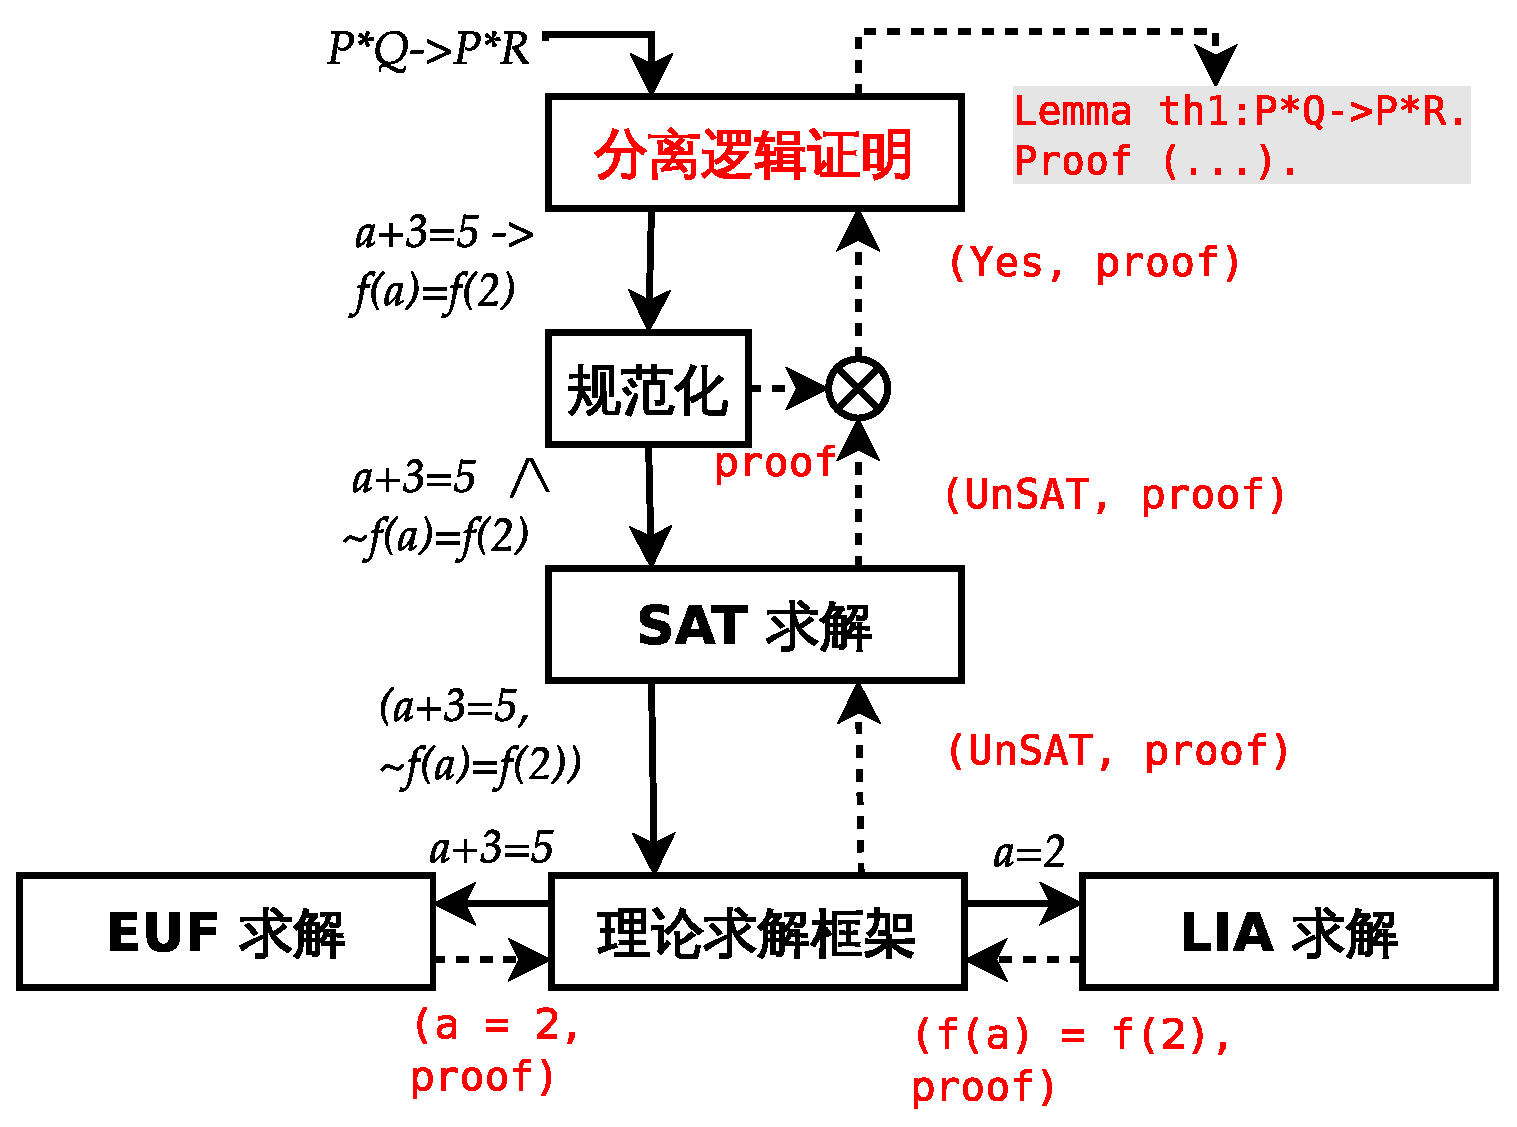
\includegraphics[width=0.9\textwidth]{stru.eps}
  \caption{证明器的结构}
  \label{struct:fig}
\end{figure}

如图\ref{struct:fig}所示,证明器逻辑上可以分成两部分。一部分是传统的基于一阶逻辑证明器;另一个部分是分离逻辑的证明器。

\subsection{分离逻辑模块所做的工作}
证明器开始运行时,最先由分离逻辑证明模块接收上一节所述的命题语言$\Pi \land \Sigma \impl \Pi' \land \Sigma'$。

接着,分离逻辑证明模块将命题化归成求证:
\begin{eqnarray}
  \vdash & \Pi \impl \Pi' \label{struct:eq1}\\
  \vdash & \Pi \land \Sigma \impl \Sigma' \label{struct:eq2}
\end{eqnarray}

\ref{struct:eq1}式是一个纯的一阶逻辑的证明过程,因此直接将该部分命题发送到一阶逻辑证明部分求证。

\ref{struct:eq2}式是一个带分离逻辑的证明过程,同时它要用到纯一阶逻辑部分的一些假设。该部分将由分离逻辑证明模块使用分离逻辑中的定理将该过程分解成求证一系列纯一阶逻辑命题,发送到一阶逻辑证明部分求证。该部分的方法在第\ref{chap:sep}章说明。

分离逻辑证明模块综合两式,就能得到命题的最终证明。

\subsection{一阶逻辑模块所做的工作}
对于每一个被发送到一阶逻辑模块的命题,首先经过命题逻辑证明模块。该模块将所有不同的公式项看作一个独立的命题变元,最终化简成为约束满足(SAT)问题,该步的具体方法在第\ref{chap:sat}章说明。

由于命题逻辑证明求解时不会关心命题公式项的具体内容,因此它在求解时会生成一系列可能否证命题的``反例''赋值。这些``反例''重新构成命题后被发送到理论整合框架。在这个框架中,命题被按照公式项分成不同的部分,送给不同的理论求解器求解。由于考察公式项的具体结构,``反例''将被一一反驳。该步具体方法在第\ref{chap:euf}、\ref{chap:lia}、\ref{chap:no}章说明。

命题逻辑证明模块综合这些反驳信息,就能得到命题的最终证明。

